\documentclass[10pt]{article}
\usepackage[a4paper,margin=2.15cm]{geometry}
\usepackage{amsmath,amssymb,mathtools}
\usepackage{booktabs}
\usepackage{microtype}
\usepackage{graphicx}
\usepackage{enumitem}
\usepackage{hyperref}
\usepackage{xcolor}
\usepackage{tikz}
\usepackage[numbers,sort&compress]{natbib}
\usetikzlibrary{arrows.meta,positioning}
\hypersetup{colorlinks=true,linkcolor=blue!45!black,citecolor=blue!45!black,urlcolor=blue!45!black}
\setlist{nosep,leftmargin=*}
\newcommand{\Ccap}{\mathcal{C}}
\newcommand{\Fset}{\mathcal{F}}

\title{\textbf{Heterogeneous Learning Systems: A Relevance Cascade for Collective Capability and Competence Evolution}}
\author{Francisco Javier Gonz\'alez Serrano\\Universidad Carlos III de Madrid}
\date{Working paper v0.2 --- October 2026}

\begin{document}
\maketitle

\begin{abstract}
Heterogeneous Learning Systems (HLS) concerns collectives whose limited,
distributed competences must be organized now and may evolve through what the
collective does. Its central scientific claim is neither that heterogeneity,
learning, nor integrated control is universally valuable. It is that a proposed
organization--development effect must pass a sequence of distinct relevance
filters before it can alter a present choice. We call this sequence the HLS
Relevance Cascade:
\[
a_t \longrightarrow S_{t+1} \longrightarrow \Ccap_{t+1}
\longrightarrow V_{t+1} \longrightarrow \text{optimal present choice}.
\]
The cascade separates state divergence (F1), capability relevance (F2), value
relevance (F3), and decision relevance (F4), with
$F4\Rightarrow F3\Rightarrow F2\Rightarrow F1$ and generally false
converses. It is a structural HLS screen, not a new dynamic-programming
theorem. We combine a static collective-capability operator with an endogenous
competence transition, reuse the former on the future state, and state the
minimal consistency condition connecting capability to value. Established
assignment, learning, and continuation-value mathematics are deliberately
imported. The scientific contribution lies in the HLS architecture, the
distinctions it requires, their null boundaries, and their assembly into one
testable collective problem. Static G1 controls establish the Beam-1
distinctions; dynamic G2 provides a staged witness for F1--F4. The result is a
compact foundation for deciding when a richer HLS model is warranted and when
the problem reduces to a simpler one.
\end{abstract}

\section{The scientific claim}

Collective problem solving is often organized around heterogeneous units: human
workers, service teams, autonomous agents, or portfolios of learned models can
differ in competence, cost, capacity, and future development. HLS studies the
system-level problem created when such a collective must both use its current
competences and determine which present actions affect its future competences.
The motivating questions are simple: \emph{who should do what?} and \emph{who
should learn what, how, and from whom?}

The contribution is not a claim that a heterogeneous, learning, or jointly
managed system dominates a simpler alternative. Nor is it a replacement for
assignment theory, learning theory, or dynamic programming. The claim is more
specific: these established components address different objects, and an HLS
analysis must preserve their order if it is to tell whether a physical
competence change can matter for a collective decision. The relevant object is
therefore the \emph{architecture of dependence} from realized action to future
state, collective capability, future value, and present choice.

This framing has two consequences. First, an equality or a null is informative:
it locates the first point at which a proposed HLS effect disappears. Second,
new machinery is unwarranted when the cascade stops early. A fixed-competence
problem can be treated as static organization; a state change that leaves
collective capability unchanged need not be promoted to a dynamic organization
problem; and a future-value difference that leaves the present optimum
unchanged does not establish decision relevance. This is a scientific criterion
for reduction, not a generic preference for more elaborate models.

\section{Beam 1: collective capability under fixed competence}

The static beam asks what a collective can achieve from its current competence
structure. Let $S$ denote the competence state, $P$ the problem or demand
conditions, $B$ the operational constraints, and $\Pi$ an admissible class of
organizational policies. For fixed $(S,P,B,\Pi)$, the feasible collective
outcome set is
\begin{equation}
\Fset_{\Pi}(S,P,B)=\{z^\pi(S,P):\pi\in\Pi_B\},
\end{equation}
and the non-dominated collective-capability frontier is
\begin{equation}
\Ccap_{\Pi}(S,P,B)=ND[\Fset_{\Pi}(S,P,B)].
\label{eq:t0}
\end{equation}
This is the static T0 object. It separates competence from feasible collective
outcomes, collective capability, realized performance, and value. Organization
is deliberately broader than routing: it is the admissible way of accessing
and using distributed competence.

This formulation imports familiar static machinery rather than recasting it as
new HLS mathematics. The organization of distributed knowledge
\citep{garicano2000}, assignment and specialization, and resource-constrained
allocation already address important parts of Beam 1. HLS supplies the common
semantic location in which their outcomes can be compared before and after
competence evolution.

For nested organizational classes, a richer class weakly expands the attainable
set. That inclusion alone is not the scientific result: it may leave the
efficient frontier unchanged (organizational sufficiency), and an expanded
frontier may still have no realized value under the specified $P$ and $B$.
Thus the Beam-1 distinction is
\begin{equation}
\text{heterogeneity}
\not\Rightarrow \text{attainable expansion}
\not\Rightarrow \text{efficient capability expansion}
\not\Rightarrow \text{organizational value}.
\label{eq:beamone}
\end{equation}
The arrows in \eqref{eq:beamone} are a sequence of questions, not a claim that
the intermediate objects are interchangeable.

\paragraph{G1: the static reference.}
G1 is a fixed-competence, two-agent/two-task ground truth for these
distinctions. It includes homogeneous and dominance nulls, crossed
specialization, resource-effectiveness trade-offs, and a budget control in
which the same competence structure has zero, then positive, then zero
organizational value. It therefore establishes only the scoped Beam-1 lesson:
organizational value is a property of $(S,P,B,\Pi)$, not of $S$ or
heterogeneity alone. G1 is not evidence about competence evolution or a claim
of novel static operations-research theory.

\section{The HLS Relevance Cascade}

\subsection{From realized action to future capability}

The minimum dynamic boundary is endogenous competence change through realized
organizational use:
\begin{equation}
S_{t+1}=F(S_t,a_t).
\label{eq:transition}
\end{equation}
The distinction between the policy and the realized action matters: the
transition is caused by what the collective does, not merely by the nominal
policy description. If the future state is independent of present action, the
system is a succession of static Beam-1 problems.

Dynamic HLS does not define a second kind of collective capability. It reuses
\eqref{eq:t0} under future operating conditions:
\begin{equation}
\Ccap_{t+1}(a_t)=
\Ccap_{\Pi^*_{t+1}}\bigl(F(S_t,a_t),P_{t+1},B_{t+1}\bigr).
\label{eq:futurecap}
\end{equation}
For alternatives $a,a'$, this permits a first distinction between a changed
state and changed efficient collective capability.

Let $V_{t+1}(S;\theta_{t+1})$ be the best future collective performance under
common future operating conditions
$\theta_{t+1}=(P_{t+1},B_{t+1},\Pi_{t+1})$ and the performance criterion of
the instantiated problem. No universal scalar HLS utility is assumed. The
minimal T4$\rightarrow$T5 consistency condition is:
\begin{equation}
\Ccap_{t+1}(a)=\Ccap_{t+1}(a')
\quad\Longrightarrow\quad
V_{t+1}(F(S_t,a);\theta_{t+1})=
V_{t+1}(F(S_t,a');\theta_{t+1}),
\label{eq:consistency}
\end{equation}
provided future conditions are common and the criterion is compatible with T0,
that is, evaluated from the same collective-capability object. Equality of
capability is therefore a sufficient null for comparative future value under
those conditions; unequal capability need not yield unequal value.

\subsection{Four successive filters}

For two present alternatives under common future conditions, the HLS Relevance
Cascade is
\begin{figure}[t]
\centering
\resizebox{\textwidth}{!}{%
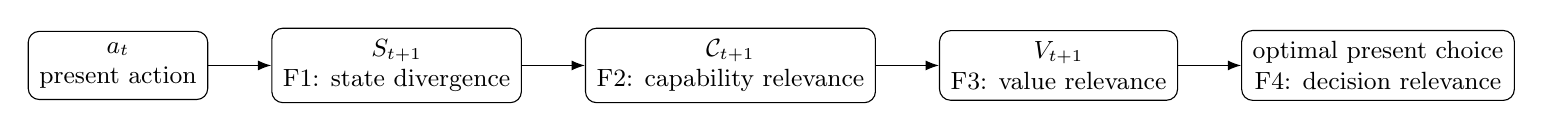
\begin{tikzpicture}[>=Latex,node distance=8mm and 8mm,
box/.style={draw,rounded corners,align=center,inner sep=4pt,font=\small}]
\node[box] (a) {$a_t$\\present action};
\node[box,right=of a] (s) {$S_{t+1}$\\F1: state divergence};
\node[box,right=of s] (c) {$\Ccap_{t+1}$\\F2: capability relevance};
\node[box,right=of c] (v) {$V_{t+1}$\\F3: value relevance};
\node[box,right=of v] (d) {optimal present choice\\F4: decision relevance};
\draw[->] (a)--(s);
\draw[->] (s)--(c);
\draw[->] (c)--(v);
\draw[->] (v)--(d);
\end{tikzpicture}
}
\caption{The HLS Relevance Cascade. Each filter asks whether the preceding
difference survives in the next HLS object.}
\label{fig:cascade}
\end{figure}
\begin{enumerate}
\item \textbf{F1 --- state divergence:} $F(S_t,a)\neq F(S_t,a')$.
\item \textbf{F2 --- capability relevance:}
  $\Ccap_{t+1}(a)\neq\Ccap_{t+1}(a')$.
\item \textbf{F3 --- value relevance:} the corresponding future values differ
  under the common future conditions.
\item \textbf{F4 --- decision relevance:} for a two-alternative present choice
  with a strict static preference, the future-value term changes the optimal
  present choice.
\end{enumerate}

The structural implication is
\begin{equation}
\boxed{F4\Rightarrow F3\Rightarrow F2\Rightarrow F1.}
\label{eq:filterorder}
\end{equation}
If F1 fails, the future states and hence capability and value coincide. If F2
fails, \eqref{eq:consistency} blocks F3. If F3 fails, no differential
continuation value can change a fixed present ranking. The converses are false
in general: a state difference can be collectively redundant; different
capabilities can be equally valuable; and a positive value difference can be
too small to reverse a strict static preference.

For the minimal two-period comparison, let $\Delta R_t(a,a')$ be the present
operational difference and $\Delta^{\mathrm{dev}}_{t+1}(a,a')$ the future-value
difference. Then
\begin{equation}
\Delta J_t=\Delta R_t+\Delta^{\mathrm{dev}}_{t+1}.
\label{eq:t6}
\end{equation}
This is ordinary continuation-value reasoning. The cascade is not a theorem
of dynamic programming and does not claim new optimization mathematics; it is
the HLS structural screen that says which competence--organization distinctions
must be retained before \eqref{eq:t6} is scientifically relevant.

\section{G2 as a staged witness}

G2 is a deliberately minimal two-agent, two-task, two-period constructive and
null reference. It uses deterministic learning by doing only to instantiate
$F$; it is neither a universal dynamic HLS model nor an empirical campaign.
Its value is that each control stops, or completes, the same cascade in
Fig.~\ref{fig:cascade}.

\begin{table}[t]
\centering
\small
\begin{tabular}{p{0.16\linewidth}p{0.28\linewidth}p{0.46\linewidth}}
\toprule
Control & Cascade status & Scoped lesson \\
\midrule
D0 & F1 blocked & No evolution: alternative actions induce the same future
state, capability, and value. \\
D1 & F1 passes; F2 blocked & Learning changes state and attainable outcomes,
but both efficient frontiers are $(0.8,0.8)$. \\
D2, $p=0$ & F2 passes; F3 blocked & Future efficient capabilities differ, but
$\Delta^{\mathrm{dev}}(0)=0$. \\
D2, $0<p<0.5$ & F3 passes; F4 not reached &
$\Delta^{\mathrm{dev}}(p)>0$, yet it does not overcome the present
operational disadvantage. \\
D2, $p>0.5$ & F4 reached & Future development value reverses the strictly
static preference. \\
\bottomrule
\end{tabular}
\caption{G2 as a staged witness for the HLS Relevance Cascade.}
\label{tab:g2}
\end{table}

In D2, the present difference and development value are
\begin{equation}
\Delta R=-0.1,\qquad
\Delta^{\mathrm{dev}}(p)=0.2p,\qquad
\Delta J(p)=-0.1+0.2p.
\label{eq:d2}
\end{equation}
Consequently, $p=0$ is the T5 null, $0<p<0.5$ exhibits value relevance without
decision relevance, $p=0.5$ is intertemporal indifference, and $p>0.5$
reaches F4. This is precisely why passing F1--F3 is not sufficient for F4.
G2 supplies a witness for the logical boundaries; it does not establish the
prevalence, robustness, or irreducibility of any dynamic organizational
arrangement.

\section{What the HLS architecture adds}

The mathematics used at each stage is intentionally familiar. Static
collective capability can draw on assignment, resource-allocation, and
organizational theories of distributed knowledge \citep{garicano2000}.
Transitions can instantiate established accounts of learning by doing,
task-specific human capital, or organizational learning
\citep{arrow1962,gibbonswaldman2004,argotemiron2011}. Once a particular state,
transition, and criterion have been specified, dynamic programming supplies
the appropriate continuation-value calculation. Competence-oriented dynamic
portfolio work and dynamic staffing already study particular operation--
development interactions \citep{gutjahr2011,borgonjon2024dynamic}.

HLS does not relabel these components as a new mathematical theory. Its
scientific contribution is their disciplined assembly around a collective
problem: (i) one static capability semantics before and after competence
evolution; (ii) realized action as the causal interface to future competence;
(iii) an explicit separation of state, capability, value, and decision
relevance; and (iv) null boundaries that identify when the composition reduces
to a simpler established problem. These are not merely a catalogue of
framework elements. Together they impose falsifiable structural requirements
on any claim that organization and competence development are consequential.

The architecture also disciplines interpretation. F4 does not imply that
centralized or irreducibly joint management is required: a sufficient
continuation signal or a modular decomposition may reproduce the same optimum.
Conversely, a failure before F4 is not an unsuccessful HLS experiment. It is a
scoped result showing which proposed dependency is absent under the stated
conditions. HLS therefore treats reduction, sufficiency, and null results as
scientifically informative outcomes.

\section{Scope and conclusion}

The foundation makes no claim of universal learning value, universal
heterogeneity value, universal superiority of dynamic organization, novel
dynamic-programming theory, or necessity of irreducibly joint management. It
does not introduce a learning mechanism, an algorithm, a new dynamic block, or
a universal scalar objective. Such additions require a prior HLS question and
must be assessed against the same relevance screen.

The central result is a compact scientific architecture for a collective with
heterogeneous and evolvable competences. Beam 1 establishes that competence,
collective capability, and realized organizational value are distinct. The
dynamic beam adds the minimum endogenous transition and reuses the same
capability operator. The HLS Relevance Cascade then makes the required
successive tests explicit: a present action must create a state difference,
that difference must affect collective capability, capability must affect
future value, and future value must affect the optimal present choice. G1 and
G2 provide minimal null and positive controls for this argument. The resulting
foundation states both when an HLS effect is substantively present and when no
richer HLS machinery is warranted.

\bibliographystyle{plainnat}
\bibliography{hls_foundations_v02}
\end{document}
